\chapter{関連研究}
\label{chap:kanren}

本節では、手書きベースWikiのコンセプトや機能に関連する興味深い研究を紹介し、それらの特徴を示しつ本研究との比較を行う。
\newpage

%手書きのメモに関する先行研究は、
%個人のメモを共有可能にするもの1
%小型デバイス上でのメモ取りを支援するもの2
%3
%等数多く存在する

%アクティブリーディングにおいてもsensing grasp等が存在する4
%同様の機能をテーブルトップ上でも行うシステムが存在する56
%

\section{手書きデータをハイパーテキストとして扱うシステム}
\label{hyperillustcreators}
手書きのメモやイラスト等の画像データに対しハイパーリンクを埋めこむ機能を持つものとして
以下のようなシステムが挙げられる。

\subsection{HyperCard}
Appleによって開発されたHyperCard\footnote{http://www.apple.com/hypercard}は、マルチメディアやリンクを埋め込んだハイパーテキストのような
コンテンツを作成できるソフトウェアである。
HyperCardのコンテンツは複数のカードから構成されたスタックという形式で運用されるが、
図\ref{fig:hypercard}のように手書きの図の上にフィールドを作成し、マウスでクリックした際に
異なるカードへの移動するという処理をHyperTalkと呼ばれるスクリプト言語で記述することで
ハイパーリンクに相当する機能を実現することができる。

\paragraph*{DrawWikiとの比較}
HyperCardでは手書きの図を含むあらゆるオブジェクトに対してカード間リンクを埋めこむことができるが、
その設定にはコーディングが必要であり敷居が高い。DrawWikiは範囲選択ツールで要素を選び、リンク先のメモ・イラスト
を設定するだけで同じ操作ができるため手数が少なく、より手軽であると言える。
またカード間は自在に移動できるが異なるマシンに置かれたスタックに対してアクセスすることができない。
DrawWikiでは全てのメモ・イラストがURLを持ったハイパーテキストであるため全世界からアクセス可能である。

\begin{figure}[H]
    \centering
    \fbox{ 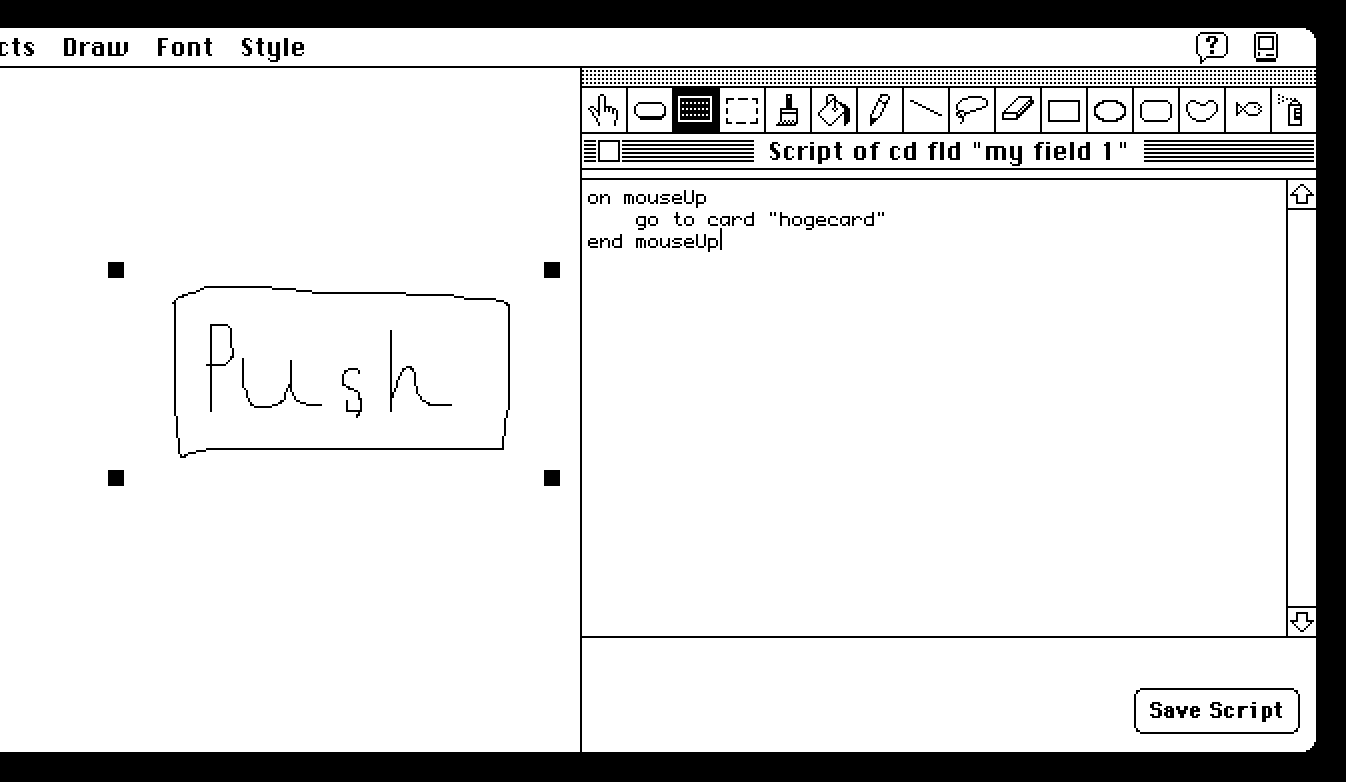
\includegraphics[width=11cm]{images/hypercard.png} }
    \caption{エミュレータ上で再現されたHyperCardの編集画面}
    \label{fig:hypercard}
\end{figure}

\subsection{Adobe Photoshop}
Adobe Systems\footnote{https://www.adobe.com/}が開発する画像編集ソフトウェアであるPhotoshop\footnote{https://www.adobe.com/jp/products/photoshop.html}には
作成した画像をHTMLファイルとして出力するオプションが存在する。設定によっては任意の領域に対してハイパーリンクを埋めこむことができる。
この時出力されるファイルは、本体となる画像とそれをオーバーレイするHTMLファイルとセットで構成される。

\paragraph*{DrawWikiとの比較}
そもそもPhotoshopはプロフェッショナル向けのツールであり、すばやく手書きメモを取るという用途に対して多機能すぎるため、大袈裟である。
また画像付きHTMLファイルとして出力した場合、各ファイルを正しい位置関係に配置したディレクトリごと配布される必要があり、
1ファイルで画像とハイパーリンクの双方を記述できるSVGと比較してポータビリティに欠ける。

\subsection{Inkscape}
The Inkscape Team\footnote{https://inkscape.org/user/teams/}によって開発されるオープンソースのベクター画像編集ソフトウェアである
Inkscape\footnote{https://inkscape.org/}はSVG画像をテキストエディタによって直接編集する機能を備える。
これにより複数の要素をグループ化し、同一のハイパーリンクを埋めこむ等の高度な操作を行うことができる。

\paragraph*{DrawWikiとの比較}
Photoshopと同様Inkscapeも手書きメモという用途に対して高機能すぎ、またSVGを直接編集するには
SVGやXMLの仕様についてよく理解している必要があるため敷居が高い。
DrawWikiではSVGの構造をユーザーが意識することなく同一の操作を実現できる。
またPhotoshopと同様サポートしている機能は画像に対するハイパーリンクの埋め込みのみで、
ホスティング等は行わない。したがって作った画像を参照可能にするためには、ユーザー自らがリンクさせる画像をサーバーに
ホスティングしなければならないため、Wikiツールとして活用するには機能不足であると言える。

\section{手書きデータによって文書の参照や管理・再利用を支援するシステム}
メモやイラストに限らず文字を書く、下線を引く、丸で囲む等の手書きデータを
文書の閲覧や検索に応用し、参照や管理・再利用に活用する試みとして以下のシステムが挙げられる。

\subsection{XLibris}
\begin{figure}[H]
    \centering
    \fbox{ 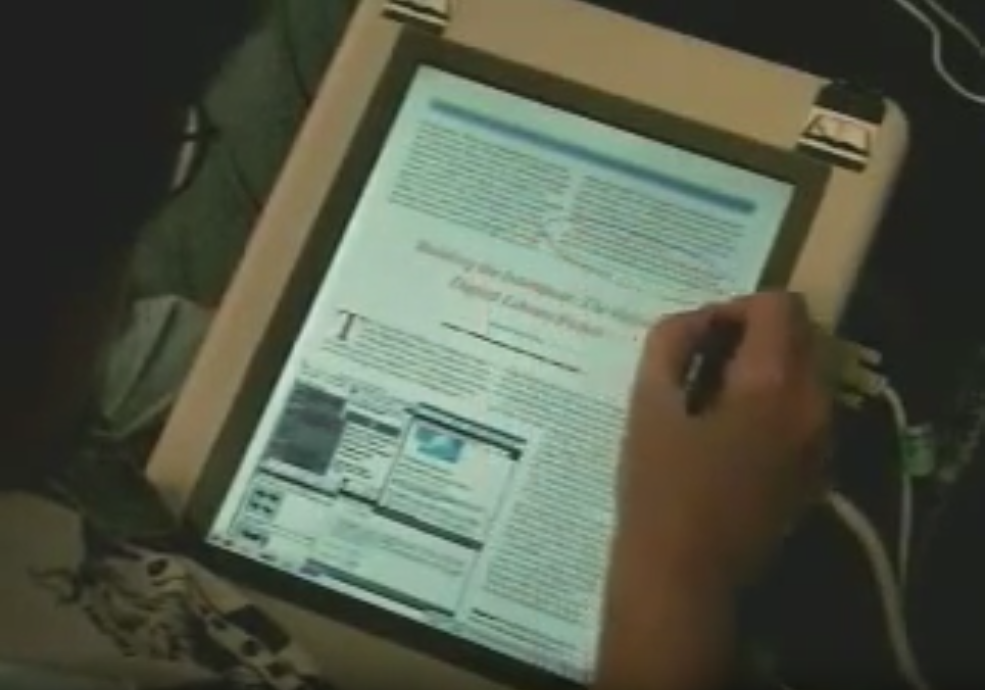
\includegraphics[width=10cm]{images/xlibris.png} }
    \caption{操作中のXLibris}
    \label{fig:xlibris}
\end{figure}
PriceらによるXLibris\cite{Price1998XLibrisTA}(図\ref{fig:xlibris})はタブレットデバイス上でActive Readingを行うことを目的としたシステムである。
スタイラスペンによって手書きの注釈やハイライトを文章中に自在に追記できるほか、
追記した部分をリンクとしてページの参照に用いたり、ハイライトされた単語や文章を検索に利用し関連資料を余白に表示する機能を備えている。

\paragraph*{DrawWikiとの比較}
メモやイラストではなく文書に追記する注釈が対象であるというコンセプトの相違があるものの、手書きの注釈がリンクとなり文書を参照しやすくなる機能や、
追記されたページを関連資料として表示する機能がActive Readingといった用途においても有用であることが示されている。

\subsection{InkSeine}
Hinckleyらによって開発されたInkSeine\cite{Hinckley2007InkSeineIS}(図\ref{inkseine})はペンインターフェースを備えたタブレットPC上での利用を想定した
Active note takingのためのシステムである。
テキスト入力も手書き文字認識によって行われる等、キーボードを使わずにペンのみで操作が完結するようUIが設計されている。
また入力した手書き文字をWebページやローカルファイルの検索に活用したり、検索結果のスクリーンショットをリンクと共にキャンバスに貼り付ける等の機能を備えており、
積極的な情報の再利用を実現している。

\paragraph*{DrawWikiとの比較}
手書きの文字を認識し、検索結果をリンクと共にノートに配置するという機能によって
ペンベースの個人用電子スクラップブックとして活用することは可能であるものの、
Wikiシステムとしての活用は想定されておらず、作成したノートのURLによる共有や
共同編集等の機能はない。

\begin{figure}[H]
    \centering
    \fbox{ 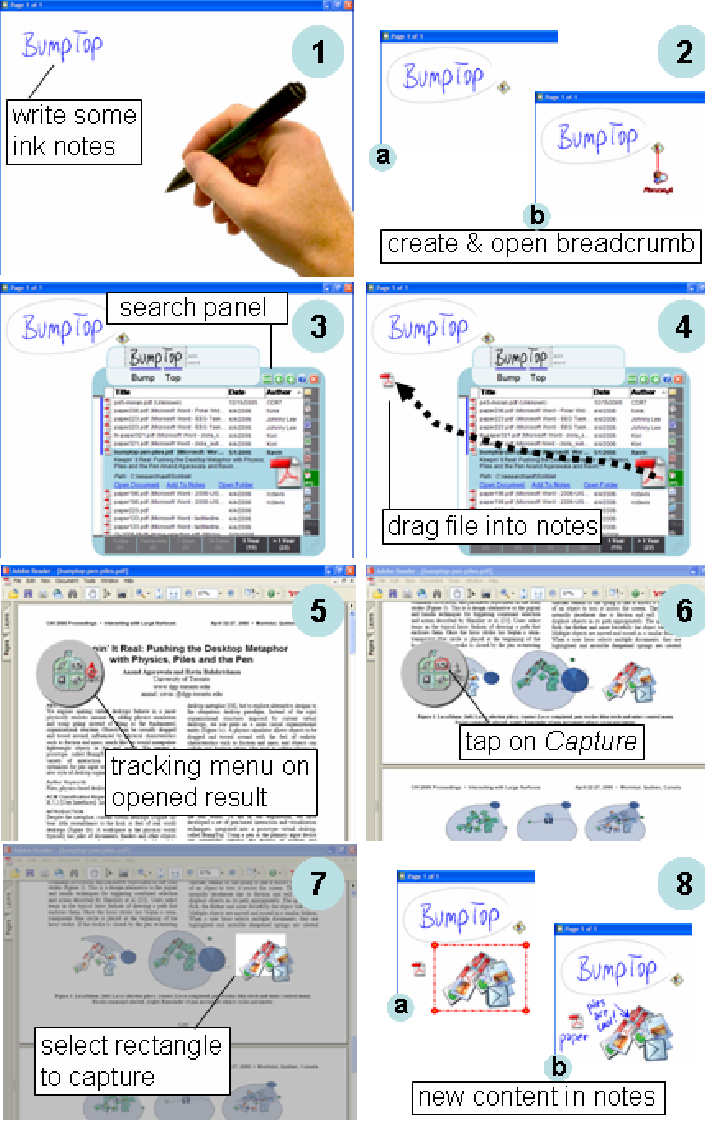
\includegraphics[width=10cm]{images/inkseine.png} }
    \caption{InkSeineの操作画面}
    \label{inkseine}
\end{figure}

\section{手書きスケッチをプロトタイピングに応用するシステム}
アプリケーションやWebサイトのUIをデザインする初期の段階ではスケッチがよく利用される\cite{Newman2000SitemapsSA}。
スケッチとしての手書きデータをそのプロトタイピングに取り入れる試みとして以下のシステムが挙げられる。

\subsection{DENIM}
\label{denim}

\begin{figure}[H] \begin{minipage}{0.5\hsize}
                         \begin{center} \fbox {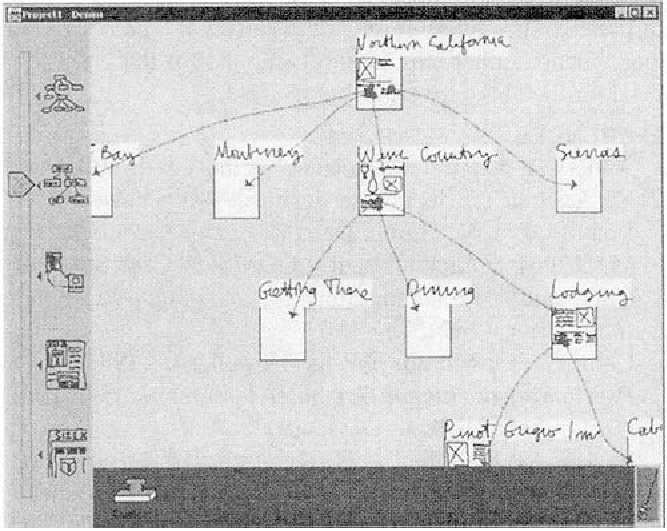
\includegraphics[width=70mm]{images/denim1.png}}
                         \end{center} \caption{DENIMの画面} \label{fig:denim1}
\end{minipage} \begin{minipage}{0.5\hsize}
                   \begin{center} \fbox {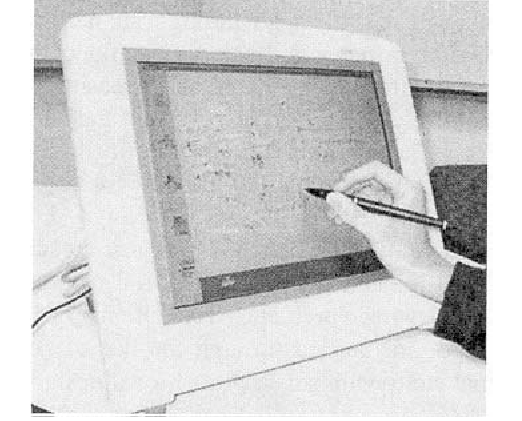
\includegraphics[width=70mm]{images/denim2.png}}
                   \end{center} \caption{操作を行うタブレット機器} \label{fig:denim2}
\end{minipage}
\end{figure}

Linらはタブレットからのスケッチを元にWebサイトのデザインやナビゲーションの設計の支援を行うシステムDENIMを開発した\cite{Lin2000DENIMFA}(図\ref{fig:denim1})。
図\ref{fig:denim2}のようなタブレット機器から操作するよう設計されており、Webページを手書きでスケッチし、それらを線で結ぶことでリンクによるナビゲーションを再現した
Webサイトのモックアップを作成することができる。またWebページの細部のデザインといった小さな視点から、複数のページ間の繋がりを俯瞰的に確認するという大きな視点までを
柔軟にカバーするために、スケッチ用キャンバスの横に視点レベルを変更可能なレンジバーが備えられており、ズーミングインターフェースの知見が取り入れられているのが
特徴である。

\subsection{SILK}
\label{silk}

\begin{figure}[H]
    \centering
    \fbox{ 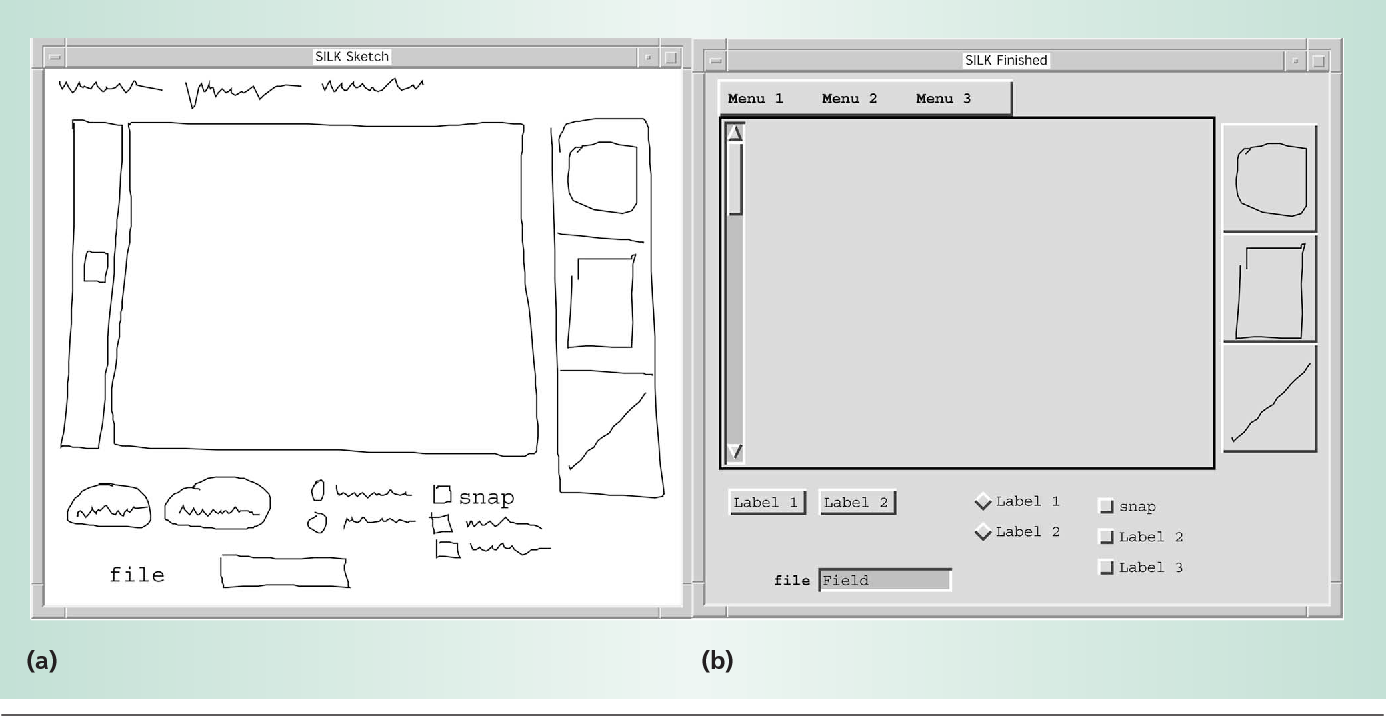
\includegraphics[width=10cm]{images/silk.png} }
    \caption{SILKの画面}
    \label{fig:silk}
\end{figure}

Landayらはスタイラスから入力した手書きデータから実際に動作するGUIを構築するSILK(Sketching Interfaces Like Krazy)というシステムを実装した
\cite{Landay2001SketchingIT}(図\ref{fig:silk})。
このシステムは手書きデータの形状からボタンやフォーム等のUIコンポーネントを類推し、配置することで動作可能なソフトウェアのプロトタイプを
構築することができる。

\paragraph*{DrawWikiとの比較}
いずれのシステム(第\ref{denim}節、第\ref{silk}節)も、ラフスケッチの段階である程度のインタラクションを再現するプロトタイプを作成可能なことが
デザインを行う上で役立つことを示している。DrawWikiはデザインを専門とするツールではないが、手書きスケッチの内部へのリンク埋め込みや、
リンク先画像のダイアログ表示といった機能を用いることで第\ref{drawiki:mockup}節のように「インタラクションを伴うプロトタイプ」として応用することができる。
したがってDrawWikiはデザインの分野においても応用可能なツールであると言える。
%さらにDrawWikiは本来のWikiとしての機能も備えているため、書き捨てることが一般的だったラフスケッチをリンクによって参照・再利用可能な活きたナレッジ
%として活用することができる。

\section{手書きスケッチの中の要素に注釈を埋め込めるシステム}
手書きのスケッチの内部に、手書きのメモ・イラストや画像、音声等のメディアを注釈として埋めこむシステムとして
以下が挙げられる。

\subsection{SketchComm}
\label{sketchcomm}

\begin{figure}[H] \begin{minipage}{0.5\hsize}
                      \begin{center} \fbox {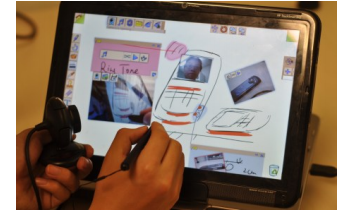
\includegraphics[width=70mm]{images/sketchcomm1.png}}
                      \end{center} \caption{} \label{fig:sketchcomm1}
\end{minipage} \begin{minipage}{0.5\hsize}
                   \begin{center} \fbox {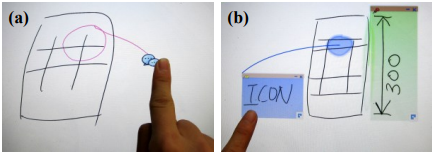
\includegraphics[width=70mm]{images/sketchcomm2.png}}
                   \end{center} \caption{} \label{fig:sketchcomm2}
\end{minipage}
\end{figure}
LiらによるSketchComm\cite{Li2012SketchCommAT}はアイデアに関するスケッチが非同期的にレビューされることを念頭に置いて設計されたシステムである(図\ref{fig:sketchcomm1})。
対面によるコミュニケーションを伴う同期的なレビューと異なり、非同期的なレビューではコンテキストが欠落する恐れがあるため、
それを補うために注釈やコメント、音声データ等をスケッチの内部に埋め込むことができる(図\ref{fig:sketchcomm2})。
これらのコンテンツはキャンバスを専有しないよう必要に応じて表示・非表示を切り替えられる。このシステムを用いた評価実験を行ったところ、「注釈を活用することでスケッチの視認性を
確保しながらも必要な情報は適宜参照できること」が実験に参加したデザイナーから高く評価されていた。またOneNote\footnote{https://www.onenote.com/}等の既存のシステム
との比較も行われており、 「同じコンセプトを表現する場合、注釈が利用できないOneNoteでは多くの情報をキャンバスに描かなければならないためスケッチが見づらくなった」「SketchCommの方がOneNoteよりも
少ない労力で多くを表現できる」という評価がなされている。

\paragraph*{DrawWikiとの比較}
DrawWikiが手書きメモ・イラストの中に埋めこむのはハイパーリンク(URL)であるが、クリックすると即座に遷移するのではなく
リンク先の画像がダイアログで表示されるため、第\ref{drawiki:mockup}節や第\ref{drawiki:zukai}節のように「表示/非表示を切り替え可能な注釈」として活用することができる。
スケッチの内部に関連する情報をあわせて保存できることがコンセプトの理解を助けることをこの研究は示しており、この機能はWikiシステムにおいても有効であると考えられる。